\documentclass{beamer}
\usepackage[utf8]{inputenc}
\usepackage{mathptmx}
\usepackage[scaled=0.9]{helvet}
\usepackage{courier}
\usepackage{listings}
\usepackage{color}

\definecolor{dkgreen}{rgb}{0,0.6,0}
\definecolor{gray}{rgb}{0.5,0.5,0.5}
\definecolor{mauve}{rgb}{0.58,0,0.82}
\definecolor{links}{HTML}{2A1B81}
\hypersetup{colorlinks,linkcolor=,urlcolor=links}
\usepackage[normalem]{ulem}
\lstset{
        frame=tb,
        language=C,
        showstringspaces=false,
        columns=flexible,
        basicstyle={\small},
        numbers=left,
        numberstyle=\tiny\color{gray},
        xleftmargin=2em,
        framexleftmargin=1.5em,
        keywordstyle=\color{blue},
        commentstyle=\color{dkgreen},
        stringstyle=\color{mauve},
        breakatwhitespace=true,
        tabsize=4,
        breaklines=true
       }
\usetheme{Madrid}
\usecolortheme{beaver}
\setbeamertemplate{navigation symbols}{} %remove navigation symbols

\title{Side Channel Analysis}
\author{Drew Monroe}

\begin{document}

\begin{frame}
\titlepage
\end{frame}

\begin{frame}
\frametitle{Outline}
\tableofcontents
\end{frame}

\section{Introduction}

\begin{frame}
    \begin{center}Traditionally, our cybersecurity talks focus on things like these...\end{center}
\end{frame}

\begin{frame}
\begin{figure}
  \centering
    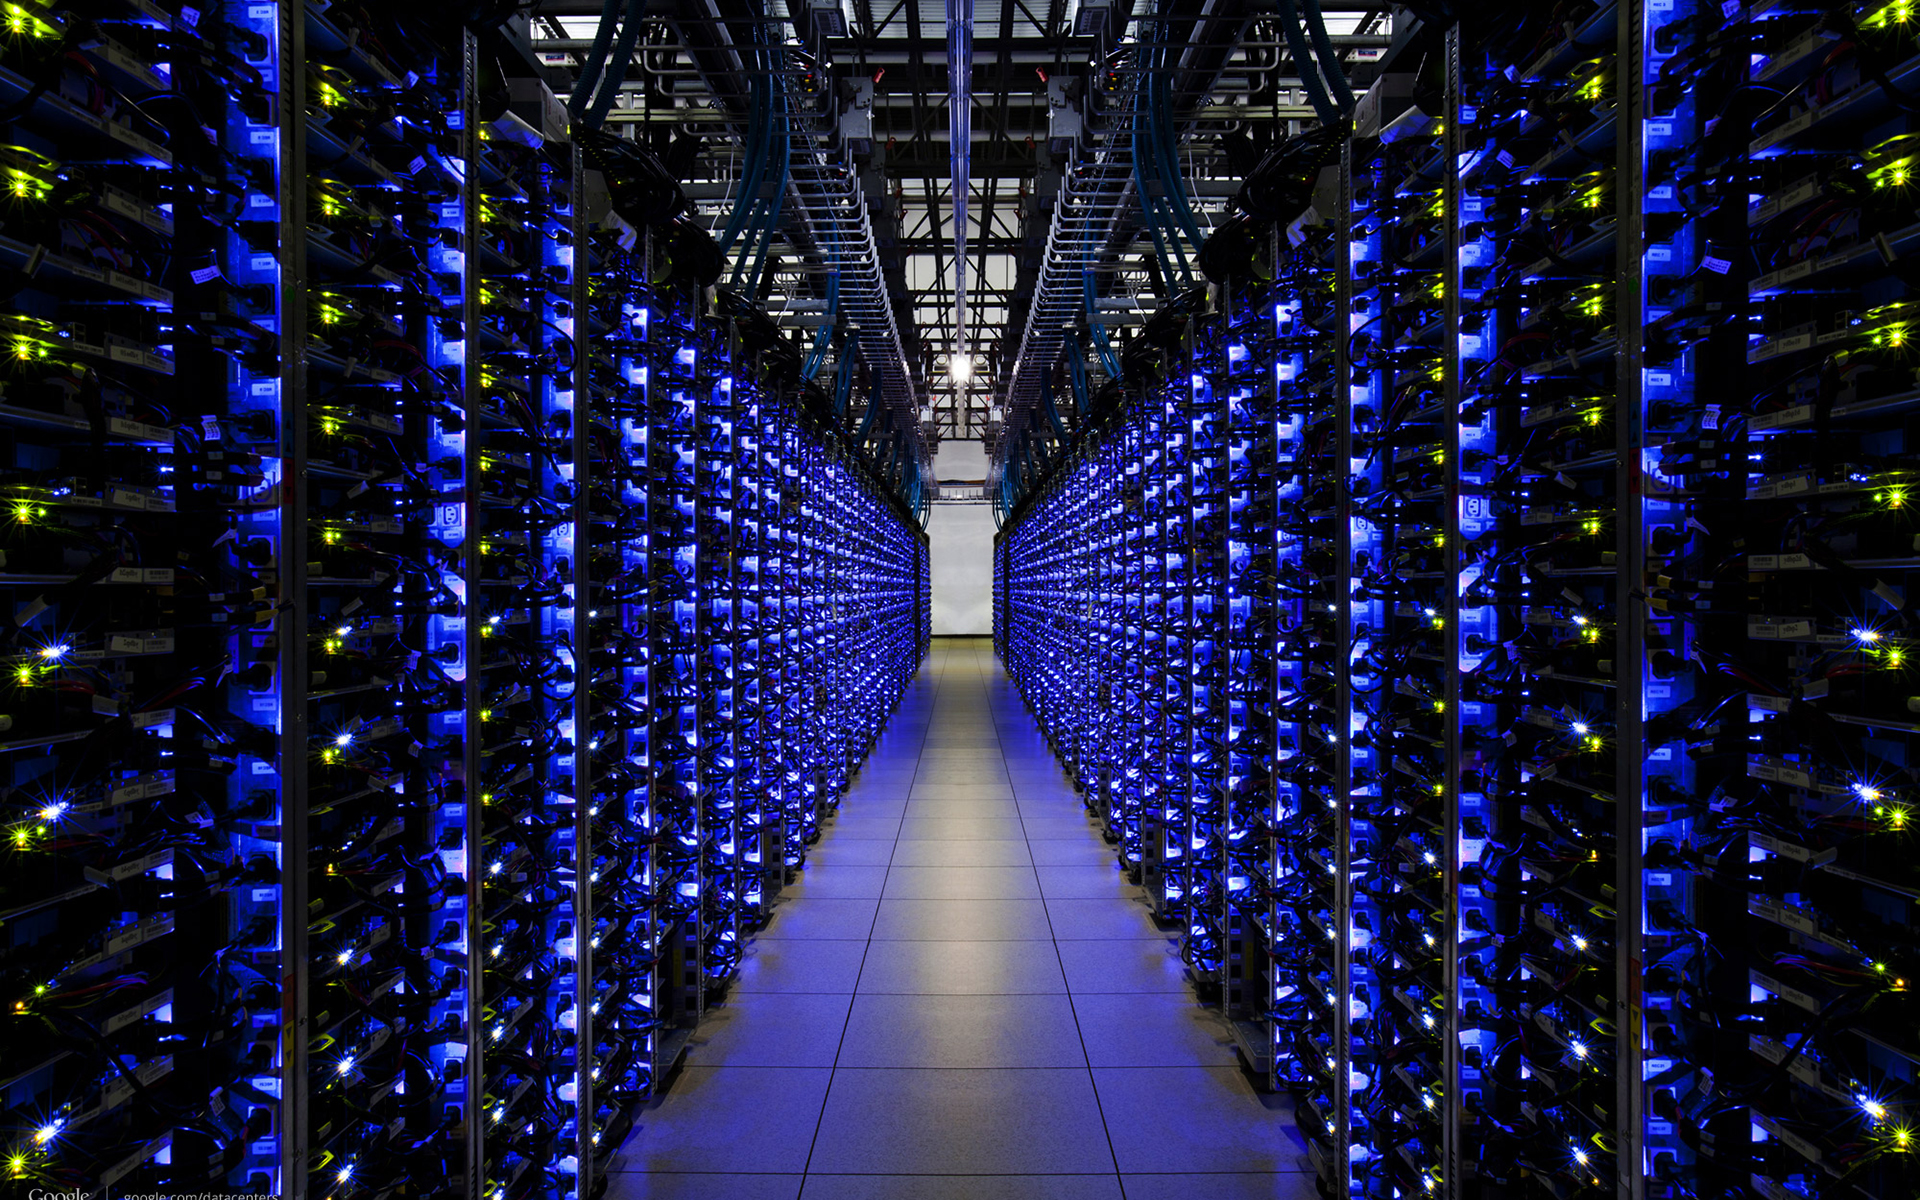
\includegraphics[width=\linewidth,height=\textheight,keepaspectratio]{images/server-room.jpg}
    \cite{ServerRoom}
\end{figure}
\end{frame}

\begin{frame}
\begin{figure}
  \centering
    
\includegraphics[width=\linewidth,height=\textheight,keepaspectratio]{images/phonesystemhackercreep.jpg}
    \cite{Hacker}
\end{figure}
\end{frame}

\begin{frame}
\begin{figure}
  \centering
    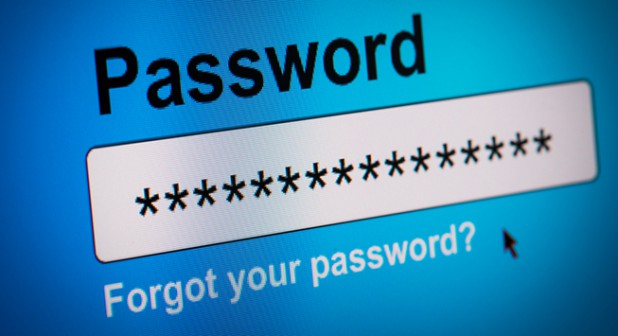
\includegraphics[width=\linewidth,height=\textheight,keepaspectratio]{images/password1-618x336.jpg}
    \cite{Password}
\end{figure}
\end{frame}

\begin{frame}
    \begin{center}But now, let's think about things like these...\end{center}
\end{frame}

\begin{frame}
\begin{figure}
  \centering
    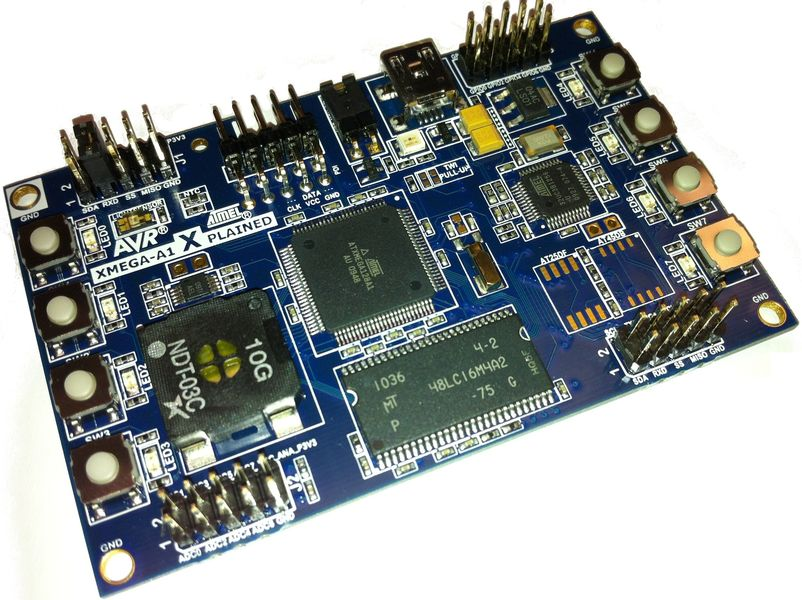
\includegraphics[scale=0.404]{images/embedded.jpg}
    \cite{Embedded}
\end{figure}
\end{frame}

\begin{frame}
    \begin{center}Your computer is made up of hardware after all!\end{center}
\end{frame}

\begin{frame}
    \begin{center}In short, what if an attacker has physical access to your system?\end{center}
\end{frame}
\section{}

\section{Information Leakage}

\begin{frame}[t]
\frametitle{Information Leakage}
\begin{itemize}
    \item You are leaking information about you behaviors all of the time!
    \begin{itemize}
        \item Sound (fans)
        \item Heat (GPS, intensive calculations, etc.)
        \item \textbf{Power}
    \end{itemize}
    \item You can think of your computer having two inputs, and two outputs
\end{itemize}
\end{frame}

\begin{frame}[t]
\frametitle{Okay, but so what?}
\begin{itemize}
    \item This information leakage can indicate what you are doing and when you are doing it.
    \begin{itemize}
        \item Think outside of computing first: your home, the pool, ambient noise
        \item Now think small scale: using a GPS, decrypting an encrypted message, hashing a password
    \end{itemize}
    \item Remember, someone has gained physical access to your system!
    They can use this information to do malicious things
\end{itemize}
\end{frame}

\begin{frame}
    \begin{center}
    Okay Drew, that's great, this sounds like it could potentially be a problem.
    But how easy is this to do?
    \end{center}
\end{frame}

\begin{frame}
    \begin{center}It's so easy, even \textbf{YOU} can do it!\end{center}
\end{frame}

\begin{frame}
\frametitle{LED Power Trace}
\begin{figure}
  \centering
    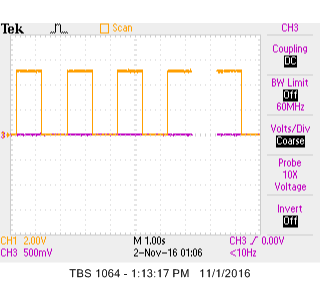
\includegraphics[width=\linewidth,height=\textheight,keepaspectratio]{images/led.png}
\end{figure}
\end{frame}

\begin{frame}
    \begin{center}
    Okay, cool, that was pretty easy!
    But that was just an LED.
    It doesn't matter if someone knows that my LED is blinking...
    \end{center}
\end{frame}

\begin{frame}[t]
\frametitle{What does this show?}
\begin{itemize}
    \item Periodically, the chip is consuming more power, and we can see when this happens.
    \item What are some things this could indicate?
        \begin{itemize}
            \item New email
            \item Voicemail
            \item Fire alarm
        \end{itemize}
\end{itemize}
\end{frame}

\begin{frame}
    \begin{center}So how could someone exploit this?\end{center}
\end{frame}

\section{Fault Injection}

\begin{frame}[t]
\frametitle{Fault Injection}
\begin{itemize}
    \item Cause a malfunction in the computer chip
    \item Goal: small errors with a large impact
    \item What causes a fault?
        \begin{itemize}
        \item Heat
        \item Radiation
        \item Electrical noise
        \item Electromagnetic pulse
        \item Changes in voltage
        \item Electrical noise
        \end{itemize}
    \item What can someone who has access to your code do? Lots of bad things...
\end{itemize}
\end{frame}

\begin{frame}
    \begin{center}Let's write some C!\end{center}
\end{frame}

\begin{frame}[fragile]
\frametitle{Password Checks}{\vspace{-3em}}
\begin{columns}[t]
\begin{column}{0.5\textwidth}
\begin{center}C\end{center}
\begin{lstlisting}
char* password = "12345";
char* hash = md5(password);
char* stored_hash = getStoredHash();

int checkPassword(char* hash, char* stored_hash)
{
    if (strcmp(hash, stored_hash) == 0)
    {
        return letUserIn();
    }
    else
    {
        return getWrecked();
    }
}
\end{lstlisting}
\end{column}

\begin{column}{0.5\textwidth}
\begin{center}MIPS\end{center}
\begin{lstlisting}[language={}]
# $a0 is the hashed password
# $a1 is the stored hashed password

checkPassword:
    bne    $a0     $a1    getWrecked
    # Do stuff because password is correct
    j      return

getWrecked:
    # Deny the user
    j      return

return:
    # pop the stack and return
\end{lstlisting}
\end{column}

\end{columns}
\end{frame}

\begin{frame}
    \begin{center}So what is wrong with this?\end{center}
\end{frame}

\begin{frame}[fragile]
\frametitle{Password Checks}{\vspace{-3em}}
\begin{columns}[t]
\begin{column}{0.5\textwidth}
\begin{center}C\end{center}
\begin{lstlisting}
char* password = "12345";
char* hash = md5(password);
char* stored_hash = getStoredHash();

int checkPassword(char* hash, char* stored_hash)
{
    if (strcmp(hash, stored_hash) == 0)
    {
        return letUserIn();
    }
    else
    {
        return getWrecked();
    }
}
\end{lstlisting}
\end{column}

\begin{column}{0.5\textwidth}
\begin{center}MIPS\end{center}
\lstset{emph={bne},emphstyle=\textbf} % janky solution to get "bne" to be bold below
\begin{lstlisting}[language={}]
# $a0 is the hashed password
# $a1 is the stored hashed password

checkPassword:
    bne    $a0     $a1    getWrecked
    # Do stuff because password is correct
    j      return

getWrecked:
    # Deny the user
    j      return

return:
    # pop the stack and return
\end{lstlisting}
\end{column}

\end{columns}
\end{frame}

\begin{frame}[fragile]
\frametitle{Password Checks}{\vspace{-3em}}
\begin{columns}[t]
\begin{column}{0.5\textwidth}
\begin{itemize}
    \item What if we just don't execute that \textbf{bne} instruction?
        \begin{itemize}
            \item Yeah right! That's not how code works!
        \end{itemize}
\end{itemize}
\end{column}

\begin{column}{0.5\textwidth}
\begin{center}MIPS\end{center}
\lstset{emph={bne},emphstyle=\sout} % janky solution to get "bne" to be bold below
\begin{lstlisting}[language={}]
# $a0 is the hashed password
# $a1 is the stored hashed password

checkPassword:
    bne    $a0     $a1    getWrecked
    # Do stuff because password is correct
    j      return

getWrecked:
    # Deny the user
    j      return

return:
    # pop the stack and return
\end{lstlisting}
\end{column}

\end{columns}
\end{frame}

\begin{frame}
    \begin{center}$\textbf{\huge{WRONG}}_\text{ \tiny{(kind of)}}$\end{center}
    \begin{center}Let's see how...\end{center}
\end{frame}

\begin{frame}[t]
\frametitle{Fault Injection Revisited}
\begin{itemize}
\item The goal of fault injection was to cause a small disturbance with a large impact
    \begin{itemize}
    \item Small disturbance: 1 instruction
    \item Large impact: Authenticate any user
    \end{itemize}
\end{itemize}
\end{frame}

\begin{frame}[t]
\frametitle{Fault Injection Revisited}
\begin{itemize}
\item Tying it all together:
    \begin{itemize}
    \item Power analysis allows us to determine when certain operations are happening
    \item If we can determine when a certain operation happens, we can know where our ``small'' disturbance will take place
    \item If we know where our disturbance will have a large impact, we can exploit this to have code perform actions that wouldn't be expected to happen
    \end{itemize}
\end{itemize}
\end{frame}

\begin{frame}
    \begin{center}Okay, you showed an example with MIPS.
    Surely that's just because it's MIPS right?
    This doesn't work with other assembly languages!
    \end{center}
\end{frame}

\begin{frame}
    \begin{center}$\textbf{\huge{WRONG}}_\text{ \tiny{(this time for sure)}}$\end{center}
\end{frame}

\begin{frame}[fragile]
\frametitle{I have this C code}
\lstset{language=C}
\lstset{lineskip=-2.75pt}
\begin{lstlisting}
#include <stdlib.h>
#include <string.h>
#include <stdio.h>

int checkPassword(char* hash, char* stored_hash)
{
    if (strcmp(hash, stored_hash) == 0) // if the strings match
    {
        return 0;
    }
    else
    {
        return 1;
    }
}

int main(int argc, const char *argv[])
{
    printf("%i\n", checkPassword("you", "me"));
    printf("%i\n", checkPassword("me", "me"));
}
\end{lstlisting}
\end{frame}


\begin{frame}[fragile]
\frametitle{And this is the relevant disassembly from gdb}
\lstset{language={}}
\lstset{escapeinside={(*}{*)}}
\begin{lstlisting}
Dump of assembler code for function checkPassword:
   0x00000000004005a6 <+0>:     push   \%rbp
   0x00000000004005a7 <+1>:     mov    \%rsp,\%rbp
=> 0x00000000004005aa <+4>:     sub    \$0x10,\%rsp
   0x00000000004005ae <+8>:     mov    \%rdi,-0x8(\%rbp)
   0x00000000004005b2 <+12>:    mov    \%rsi,-0x10(\%rbp)
   0x00000000004005b6 <+16>:    mov    -0x10(\%rbp),\%rdx
   0x00000000004005ba <+20>:    mov    -0x8(\%rbp),\%rax
   0x00000000004005be <+24>:    mov    \%rdx,\%rsi
   0x00000000004005c1 <+27>:    mov    \%rax,\%rdi
   0x00000000004005c4 <+30>:    callq  0x400440 <strcmp@plt>
   0x00000000004005c9 <+35>:    test   \%eax,\%eax
   (*\bfseries 0x00000000004005cb*) <+37>:    jne    0x4005d4 <checkPassword+46>
   0x00000000004005cd <+39>:    mov    \$0x0,\%eax
   0x00000000004005d2 <+44>:    jmp    0x4005d9 <checkPassword+51>
   0x00000000004005d4 <+46>:    mov    \$0x1,\%eax
   0x00000000004005d9 <+51>:    leaveq
   0x00000000004005da <+52>:    retq
End of assembler dump.
\end{lstlisting}
\end{frame}

\begin{frame}
    \begin{center}Okay, having code just skip instructions sounds scary.
    But that's just academic theory right?
    That can't be done in pratice... right?
    \end{center}
\end{frame}

\begin{frame}
    \begin{center}$\textbf{\huge{WRONG}}$\end{center}
\end{frame}

\begin{frame}
\frametitle{Trigger}
\begin{itemize}
\item When talking about power and voltage, a trigger is a spike that is reliably produced at a given time
\item Used to determine when to start attacking the code
\end{itemize}
\end{frame}

\begin{frame}
\frametitle{Hashing}
\begin{itemize}
\item Takes a set amount of time
    \begin{itemize}
    \item Trigger on the start of the hash/when the password is sent
    \end{itemize}
\item Wait for the amount of time that the hash takes
\item Fluctuate power to obtain unexpected behavior after the hashing is completed
\end{itemize}
\end{frame}

\begin{frame}
    \begin{center}And now all we need is a way to send extra power to the board and a little python code\end{center}
\end{frame}

\begin{frame}
    \begin{center}\underline{\href{https://github.com/amuramatsu/dwf/tree/master/examples}{A quick google search yields}}\end{center}
\end{frame}

\begin{frame}
    \begin{center}Well that was easy...\end{center}
\end{frame}

\begin{frame}[fragile]
\frametitle{Pseudo-python code that doesn't actually work}
\lstset{language=Python}
\begin{lstlisting}
# import the libraries to do the things
import powertrace
# set trigger
trigger.set(VOLTAGE)
trigger.wait()
# start power fluctuations at different times
for x in range(0, 1, .1):
    # fluctuate the power
    for y in range(3, 5, .1):
        time.sleep(TIME_HASH_TAKES - SMALL_AMOUNT)
        power.set(y)
        time.sleep(JUST_LONG_ENOUGH_TO_AFFECT_THINGS)
        power.set(NORMAL_POWER)
        # check to see if we broke things
        reset()
\end{lstlisting}

\end{frame}

\section{Real Life Examples}

\begin{frame}[t]
\frametitle{Real Life Examples}
\begin{itemize}
    \item Attacks against smart cards
    \item Can be used to break mathematically secure crypto!!
        \begin{itemize}
        \item AES
        \item DES
        \item SSL
        \end{itemize}
    \item I've attacked embedded devices (with permission!)
        \begin{itemize}
            \item (Ask me about it if you want to know more)
        \end{itemize}
\end{itemize}
\end{frame}

\begin{frame}
\begin{center}This can be used to break mathematically secure crypto!\end{center}
\end{frame}

\begin{frame}[t]
\frametitle{Okay, now I'm terrified. How do I protect against this??}
\begin{itemize}
\item Perform multiplce calculations at one to cancel out traces
\item Multiple checks
    \begin{itemize}
        \item Faulting once can be tough, doing each one makes it more and more difficult
    \end{itemize}
\item Use a different algorithm that leaks less information
\item Add noise
\item Onboard brownout detection (which only kind of works)
\end{itemize}
\end{frame}

\section{Prevention}

\begin{frame}[t]
\frametitle{Okay, now I'm terrified. How do I protect against this??}
\begin{itemize}
\item Realisitcally, you don't need to worry about this in most cases (if you're not working with embedded devices)
\item HOWEVER: When dealing with things that are sensitive, especially around embedded devices, choose good algorithms!
    \begin{itemize}
        \item NSA Suite B
        \item NEVER, EVER, EVER ROLL YOU OWN CRYPTO!!
    \end{itemize}
\end{itemize}
\end{frame}

\begin{frame}[t]
  \frametitle{Want to know more about the things that I referenced?}
  \begin{itemize}
    \item\underline{\href{http://infosecwriters.com/text_resources/pdf/Known_Attacks_Against_Smartcards.pdf}{Attacks on smart cards}}
    \item\underline{\href{http://csrc.nist.gov/groups/SMA/ispab/documents/minutes/2006-03/E_Barker-March2006-ISPAB.pdf}{NSA Suite B}}
    \item\underline{\href{https://www.youtube.com/watch?v=bHncSnHQleY}{Intro talk at Cal Poly Tech}}
    
  \end{itemize}
\end{frame}

\begin{frame}
    \begin{center}Questions?\end{center}
\end{frame}

\appendix

\begin{frame}[allowframebreaks]
  \frametitle{References}
    
  \begin{thebibliography}{10}
    
 \setbeamertemplate{bibliography item}[online]

    \bibitem{ServerRoom}
    Server-Room
    \newblock
    \url{http://www.lukecjdavis.com/wp-content/uploads/2014/01/server-room.jpg}
    
    \bibitem{Hacker}
    Hacker
    \newblock
    \url{http://teamextenda.com/blog/wp-content/uploads/2014/11/phonesystemhackercreep.jpg}
    
    \bibitem{Password}
    Password
    \newblock
    \url{http://now.avg.com/wp-content/uploads/2014/05/password1-618x336.jpg}
    
    \bibitem{Embedded}
    Embedded Device
    \newblock
    \url{http://www.rcs.ei.tum.de/fileadmin/_processed_/csm_Foto_1_03_f24f1b0932.jpg}

  \end{thebibliography}
\end{frame}

\end{document}
